\documentclass{article}
\usepackage[T1]{fontenc}
\usepackage{lato}
\usepackage{graphicx}
\usepackage[unicode=true]{hyperref}
\RequirePackage{polski}
\graphicspath{ {./images/} }

\title{Laboratorium przetwarzanie obrazów}
\date{}
\author{Radosław Piotrowicz}


\begin{document}
\maketitle

\begin{center}
    \large{ Informacje potrzebne do implementacji }
\end{center}

\newpage
\tableofcontents
\newpage

\section{Gdzie znajdują się interesujące nas rzeczy.}
W każdym pliku z algorytmem należy zaimplementować metodę \textbf{AlgorithmFunction}. Wyjątek stanowią algorytmy z labów 4. Tam implementacja wygląda trochę inaczej.
\newline
\textbf{Jeżeli jakiś algorytm zawiera parametry, to znajdują się one w pliku nagłówkowym <nazwa>.hpp.}
\newline
Ponadto Clasa Alorithm, po której dziedziczą wszystkie algorytmy zawiera kilka metod pomocniczych, z których można korzystać.

\subsection{Laby 1}
\begin{itemize}
    \item Negative.cpp
    \item Brighten.cpp
    \item Contrast.cpp
    \item Logarithm.cpp
    \item Exponentiation.cpp
    \item LeveledHistorgram.cpp
    \item Masking.cpp
    \item Mixing.cpp
\end{itemize}

\subsection{Laby 2}
\begin{itemize}
    \item Binarization.cpp
\end{itemize}

\subsection{Laby 3}
\begin{itemize}
    \item LinearFilter.cpp
    \item MedianFilter.cpp
\end{itemize}

\subsection{Laby 4}
\textbf{UWAGA} tutaj jest lekka zmiana w implementacji funkcje erozji i dylatacji znajdują się w MorphologicAlgorithm.cpp (mogą zostać potem wykorzystane przy otwarciu i zamknięciu)! Pozostałe algorytmy implementujemy normalnie.
\begin{itemize}
    \item MorphologicAlgorithm.cpp (tutaj należy uzupełnić metody \textbf{ErosionFunc} oraz \textbf{DilatationFunc})
    \item Erosion.cpp (pomijamy)
    \item Dilatation.cpp (pomijamy)
    \item Opening.cpp
    \item Closing.cpp
    \item ContourInner.cpp
    \item ContourOuter.cpp
\end{itemize}

\subsection{Laby 5}
\begin{itemize}
    \item Skeletonization.cpp
\end{itemize}

\subsection{Laby 6}
\begin{itemize}
    \item Hought.cpp
\end{itemize}


\section{Co jest potrzebne przy implementacji algorytmu}
Każdy algorytm jest wykonywany w oddzielnym wątku, aby program był responsywny w związku z czym.
Każdy algorytm musi mieć w sobie 2 wywołania:
\begin{itemize}
    \item CopyToLocalVariable - na początku (kopiuje obraz do lokalnej zmiennej copy)
    \item SaveToOutput - na końcu (zapisuje lokalną kopię z powrotem)
\end{itemize}

\textbf{W każdym algorytmie są one umieszczone proszę swój kod umieścić pomiędzy!}


\subsection{Opcjonalne elementy}
Można też opcjonalnie dodać odświeżanie i możliwość przerwania wykonywania.
\newline
\textbf{ Natomiast nie jest to wymagane.}

Automatyczne odświeżanie można włączyć w zakładce Ustawienia.
Tam również można ustawić co ile sekund ma się odświeżać
/newline
Na obrazku \ref{funkcja} przedstawione jest jak korzystać z opisanych tu funkcji.

\newpage

\begin{figure}[htbp!]
    \centering
    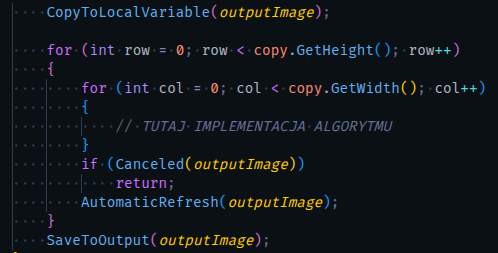
\includegraphics[width=0.8\textwidth]{Func.png}
    \caption{Przykład wykorzystania}
    \label{funkcja}
\end{figure}

\section{Opis klas i przydatnych metod}

\subsection{Klasa Algorithm}
Jest to klasa, na której bazują wszystkie algorytmy, przydatne metody w tej klasie to:
\begin{itemize}
    \item void ParamsMenu() - metoda zawierająca elementy menu do ustawienia parametrów.
    \item void AlgorithmFunction(Image *outputImage) - \textbf{funkcja algorytmu tutaj uzupełnić kod}
    \item void ResetToDefaults() - restart parametrów do wartości bazowej
    \item void Save(std::ofstream\& file) - zapis parametrów do pliku (opcjonalne)
    \item void Load(std::ifstream\& file) - wczytanie parametrów z pliku (opcjonalne)
    \item void CopyToLocalVariable(Image *outputImage) - \textbf{musi się znaleźć w funkcji algorytmu na początku}
    \item void SaveToOutput(Image *outputImage) - \textbf{musi się znaleźć w funkcji algorytmu na końcu}
    \item bool Canceled(Image *outputImage) - używamy, jeżeli chcemy móc przerwać wykonywanie algorytmu (opcjonalne)
    \item void AutomaticRefresh(Image *outputImage) - używamy, jeżeli chcemy móc odświeżyć obrazek wyjściowy w trakcie przetwarzania (opcjonalne)
    \item void ManualRefresh(Image *outputImage) - podobnie jak metoda powyżej, ale tutaj program nie będzie robił tego automatycznie po włączeniu opcji (opcjonalne)
\end{itemize}

Zawiera również takie zmienne jak:
\begin{itemize}
    \item bool autoRefresh - informuje program w jaki sposób odświeżyć (automatycznie - program ma to zrobić, ręcznie - programista decyduje kiedy)
    \item std::string algorithmName - nazwa algorytmu wyświetlana w menu wyboru algorytmów
    \item Image copy - \textbf{lokalna kopia obrazu, na której pracujemy}
\end{itemize}

\subsection{Klasa MorphologicAlgorithm}
Jest to klasa pośrednia, na której bazują algorytmy z labów 4.
Nowe metody to:
\begin{itemize}
    \item void CalculateOffsets() - jeżeli chcemy aby element przeszedł po obrazie jak najdokładniej, można policzyć jego maksymalną odległość od każdej granicy ta metoda to robi (opcjonalne)
    \item void ErosionFunc(Image *outputImage) - \textbf{tutaj implementowana będzie erozja} (może być ponownie wykorzystane przy otwarciu i zamknięciu)
    \item void DilatationFunc(Image *outputImage) - \textbf{tutaj implementowana będzie dylatacja} (może być ponownie wykorzystane przy otwarciu i zamknięciu)
\end{itemize}

Użyteczne nowe zmienne to:
\begin{itemize}
    \item int elementSize - rozmiar elementu strukturalnego
    \item bool element3x3[3][3] - element o wymiarach 3x3
    \item bool element5x5[5][5] - element o wymiarach 5x5
    \item bool element7x7[7][7] - element o wymiarach 7x7
    \item Image copyRead - \textbf{kopia do odczytu, bo są to operacje kontekstowe}
    \item int32\_t offsetLeft = 0 - minimalna odległość od lewej granicy obrazu, obliczone przez metodę \textbf{void CalculateOffsets()}
    \item int32\_t offsetRight = 0 - minimalna odległość od prawej granicy obrazu, obliczone przez metodę \textbf{void CalculateOffsets()}
    \item int32\_t offsetTop = 0 - minimalna odległość od górnej granicy obrazu, obliczone przez metodę \textbf{void CalculateOffsets()}
    \item int32\_t offsetBottom = 0 - minimalna odległość od dolnej granicy obrazu, obliczone przez metodę \textbf{void CalculateOffsets()}
    \item int32\_t elemntCopy[7][7] - kopia elementu może być wykorzystane w  głównej funkcji \textbf{Ustawiana jest w metodzie void CalculateOffsets()}
\end{itemize}

\subsection{Klasa Image}
Klasa Image jest kontenerem na obrazy, które będziemy przetwarzać.
\newline
Najbardziej interesuje nas w niej SDLSurface, czyli struktura z informacjami o pikselach w obrazie.
\newline
\textbf{UWAGA, jeżeli jakaś metoda ma wersje z końcówką NoTexture to proszę korzystać z tej wersji z tą końcówką!}
\newline
Zawiera takie przydatne metody jak:
\begin{itemize}
    \item void CopyNoTexture(Image \&other) - kopiuje zawartość danego obrazu
    \item int32\_t SetSourceImageNoTEXTURE(std::filesystem::path path) - ustawia zawartość image na obraz o podanej ścieżce (lepiej jest korzystać z menu do wczytania)
    \item Pixel GetPixel(int col, int row) - zwraca Strukturę Pixel z informacjami o pikselu w danym punkcie
    \item void SetPixel(int col, int row, Pixel pix) - ustawia pixel w danym punkcie na podany
    \item void SetPixelWhite(int col, int row) - ustawia pixel w danym punkcie na kolor biały
    \item void SetPixelBlack(int col, int row) - ustawia pixel w danym punkcie na kolor czarny
    \item int GetWidth() - zwraca szerokość obrazu
    \item int GetHeight() - zwraca wysokość obrazu
    \item int GetPixelCount() - zwraca ilość pikseli
    \item float* GetLightValues() - zwraca tablice float o długości 256 z wartościami jasności (są też wersje dla poszczególnych składowych)
    \item float* GetDistributor() - zwraca tablice float o długości 256 z wartościami dystrybuanty (są też wersje dla poszczególnych składowych)
    \item void CopyNormalisedBrightnessHistogram(float *dst) - kopiuje histogram (unormowany do wartości 0.0 - 1.0) do podanej tablicy
    \item bool NoSurface() - czy obraz zawiera poprawnie zainicjowane SDLSurface (jeśli nie to źle)
    \item void SetBlankSurfaceNoTexture(int width, int height) - ustaw obraz na biały prostokąt o wymiarach
    \item void RefreshPixelValuesArrays() - odśwież tablice z histogramami i dystrybuantami (po poprawnym zakończeniu wątku z algorytmem wątek główny automatycznie odświeży)

\end{itemize}

\subsection{Struktura Pixel}
Ta struktura zawiera wartości R, G, B oraz jasność piksela.
\newline
\textbf{Należy pamiętać, że gdy modyfikujemy piksel, należy ustawić wszystkie 3 składowe.}
\newline
\textbf{WARTOŚĆ JASNOŚCI JEST TYLKO DO ODCZYTU. METODA SetPixel NIE BIERZE JEJ POD UWAGĘ.}

\end{document}

\section{Uwagi końcowe}
Kilka innych informacji, które mogą się przydać:
\begin{itemize}
    \item Aby wyłączyć zapisywanie i wczytywanie należy zakomentować \textbf{#define LOAD_AND_SAVE 1} w pliku \textbf{App.hpp}. 
    \item Częstym błędem w implementacji niektórych algorytmów jest dzielenie całkowite zamiast rzeczywistego.
    \item Niektóre operacje są kontekstowe, potrzebna jest do nich dodatkowa kopia (znajduje się ona w pliku nagłówkowym danego algorytmu jako zmienna).
\end{itemize}
